\documentclass[a4paper,12pt]{article}

%%% Работа с русским языком
\usepackage{cmap}					% поиск в PDF
\usepackage{mathtext} 				% русские буквы в формулах
\usepackage[T2A]{fontenc}			% кодировка
\usepackage[utf8]{inputenc}			% кодировка исходного текста
\usepackage[english,russian]{babel}	% локализация и переносы
\usepackage{xcolor}
\usepackage{hyperref}
 % Цвета для гиперссылок
\definecolor{linkcolor}{HTML}{799B03} % цвет ссылок
\definecolor{urlcolor}{HTML}{799B03} % цвет гиперссылок

\hypersetup{pdfstartview=FitH,  linkcolor=linkcolor,urlcolor=urlcolor, colorlinks=true}

%%% Дополнительная работа с математикой
\usepackage{amsfonts,amssymb,amsthm,mathtools} % AMS
\usepackage{amsmath}
\usepackage{icomma} % "Умная" запятая: $0,2$ --- число, $0, 2$ --- перечисление

%% Номера формул
%\mathtoolsset{showonlyrefs=true} % Показывать номера только у тех формул, на которые есть \eqref{} в тексте.

%% Шрифты
\usepackage{euscript}	 % Шрифт Евклид
\usepackage{mathrsfs} % Красивый матшрифт

%% Свои команды
\DeclareMathOperator{\sgn}{\mathop{sgn}}

%% Перенос знаков в формулах (по Львовскому)
\newcommand*{\hm}[1]{#1\nobreak\discretionary{}
{\hbox{$\mathsurround=0pt #1$}}{}}
% графика
\usepackage{graphicx}
\graphicspath{{pictures/}}
\DeclareGraphicsExtensions{.pdf,.png,.jpg}
\author{Бурмашев Григорий, БПМИ-208}
\title{Матан, дз -- 3}
\date{\today}
\begin{document}
\maketitle
\clearpage

\section*{Номер 1}
\begin{center}
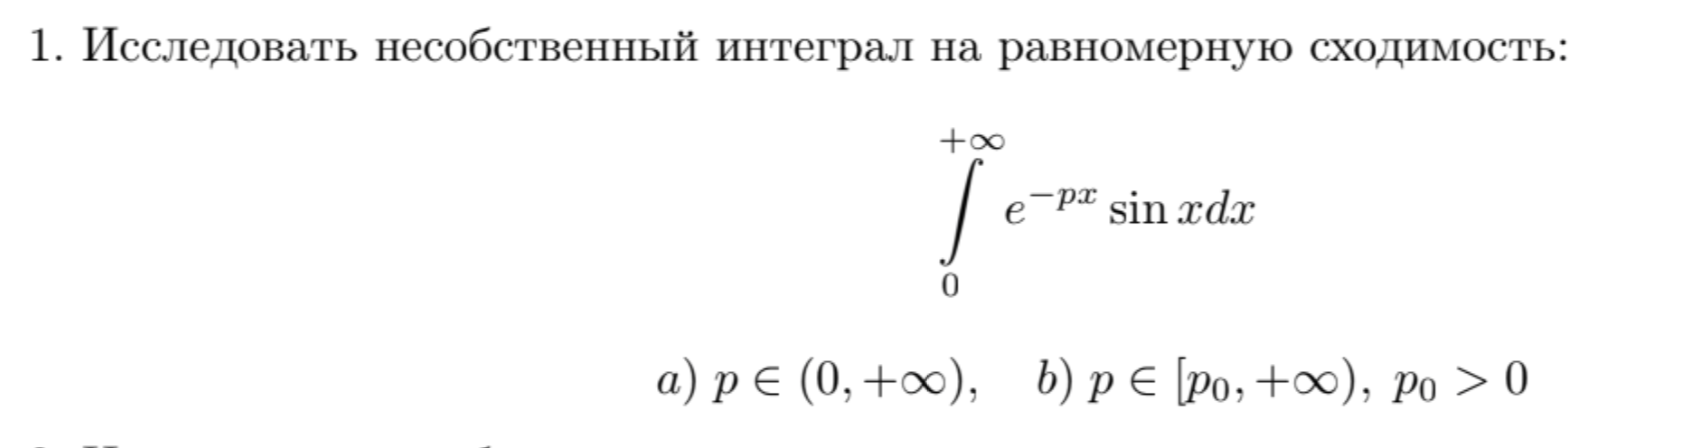
\includegraphics[scale=0.4]{1.png}
\end{center}
\subsection*{a)}
Воспользуемся методом граничной точки, подставим $p = 0$ и получим:
\[
\int_0^{\infty} e^{-0x} \sin x dx = \int_0^{\infty}  \sin x dx = - \cos x \Bigg|_0^{\infty} 
\]
Этот интеграл расходится, значит по методу граничной точки несобственный интеграл не может сходиться равномерно

\subsection*{b)}
Воспользуемся методом Вейерштрасса, начнем зажимать нашу функцию. Во первых $| \sin x | \leq 1$, во вторых $e^{-px}$ убывает, значит можем зажать левой границей для $p$, т.е $p_0$:
\[
\left|
e^{-px} \sin x 
\right|
 \leq 
\left|
e^{-px} \cdot 1
\right|
\leq 
e^{-px}
\leq 
e^{-p_0 x}
\]
Смогли ограничить, теперь посмотрим на интеграл от этой функции:
\[
\int_0^{\infty} e^{-p_0 x}  dx= 
\left(
-\frac{e^{-p_0 x}}{p}
\right)
\Bigg|_0^{\infty} 
= 
0 
+ \frac{1}{p_0} 
=
\frac{1}{p_0} 
\]
Интеграл сходится, значит по признаку Вейерштрасса наш несобственный интеграл сходится равномерно
\begin{center}
\textbf{Ответ:} a) расходится, б) сходится 
\end{center}
\clearpage
\section*{Номер 2}
\begin{center}
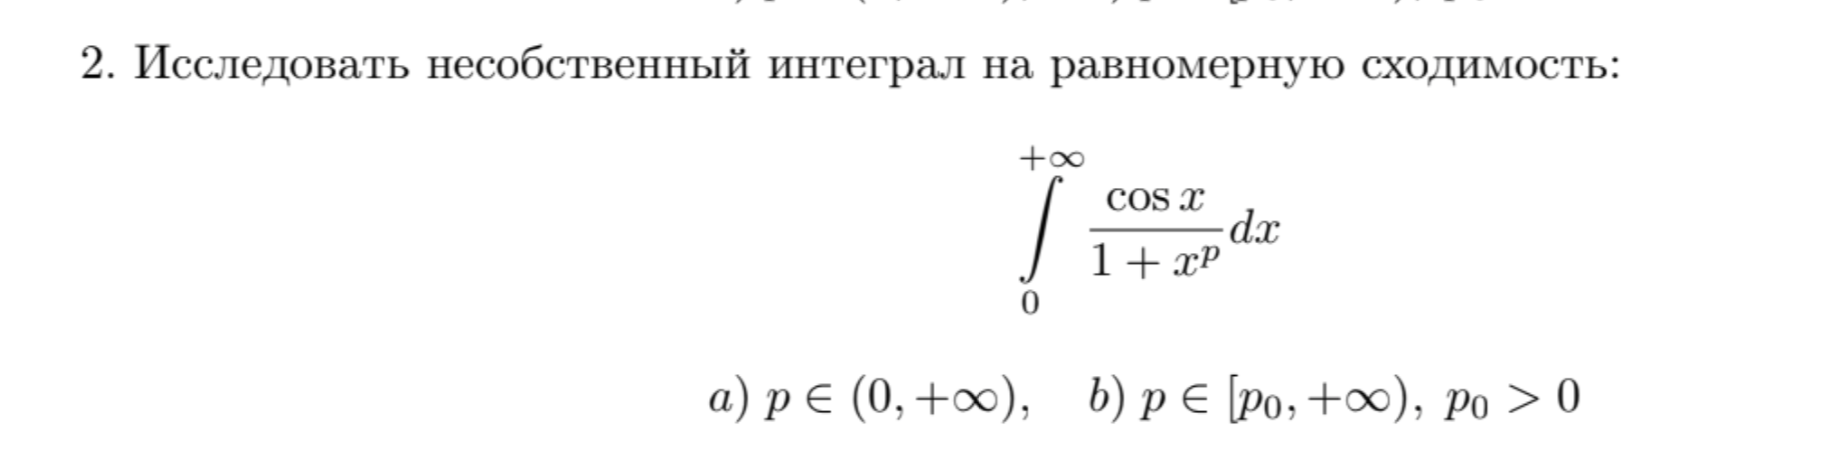
\includegraphics[scale=0.4]{2.png}
\end{center}
\subsection*{a)}
Делаем аналогично первому номеру, берем граничную точку $p = 0$ и получаем:
\[
\int_0^{+\infty} \frac{\cos x }{1 + 1} = \int_0^{+\infty} \frac{\cos x }{2}
\]
Интеграл расходится, значит несобственный интеграл не может сходиться равномерно
\subsection*{b)}
Тут хорошо можно разбить на две функции, пусть:
\[
f = \cos x, g = \frac{1}{1 + x^p}
\]
Теперь анализируем функции, попробуем по Дирихле посмотреть:
\[
\forall A > 0 \; : \; 
\left|
\int_0^A \cos x dx 
\right|
=
\left|
\sin x \Bigg|_0^A
\right|
=
\left|
\sin A - 0 
\right|
=
\left|
\sin A
\right|
\leq 1 
\]
Теперь проверяем условия для $g$, для проверки монотонности посмотрим на производную:
\[
g' = - \frac{p \cdot x^{p - 1}}{(1 + x^p)^2}
\]
Производная отрицательная, значит $g$ монотонно убывает. Далее смотрим $\rightrightarrows$ (супремум будет в $p_0$ (слева) из-за убывания функции):
\[
\underset{[p_0, +\infty]}{\sup} \left| \frac{1}{1 + x^p }\right| \overset{?}{\underset{x \rightarrow +\infty}{\longrightarrow}}  0
\]
\[
\underset{[p_0, +\infty]}{\sup} \left| \frac{1}{1 + x^p }\right| = \lim_{
x \rightarrow +\infty}
\left|
\frac{1}{1 + x^{p_0}}
\right|
=
0
\]
Отсюда:
\[
g \overset{[p_0, +\infty]}{\rightrightarrows }0, x \rightarrow +\infty
\]
Выполняются все условия для признака Дирихле, а значит есть равномерная сходимость
\begin{center}
\textbf{Ответ:} a) расходится, б) сходится 
\end{center}

\clearpage
\section*{Номер 3}
\begin{center}
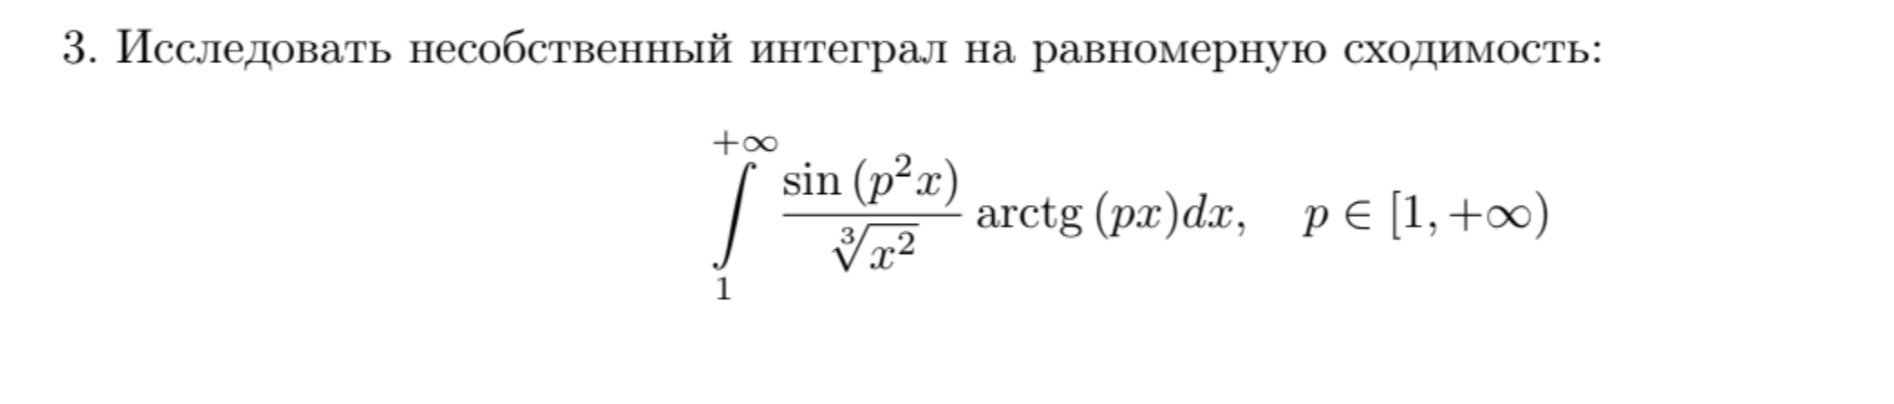
\includegraphics[scale=0.4]{3.png}
\end{center}
Опять разбиваем на две функции, пусть:
\[
f = \frac{\sin (p^2 x)}{\sqrt[3]{x^2}}, g = \arctg(px)
\]
$f$ достаточно сложная, попробуем по Абелю, сначала разберемся с более простой функцией $g$, $g$ ограничена (ибо это арктангенс), ну и монотонна (ибо это арктангенс). Теперь будем смотреть на $f$, её тоже разобьем на две функции:
\[
f_1 = \sin(p^2 x), f_2 = \frac{1}{\sqrt[3]{x^2}}
\]
\[
\forall A > 1 \; : \; 
\left|
\int_1^{A} \sin (p^2 x) \cdot \frac{1}{p^2}
\right|
= 
\begin{bmatrix}
p \in [1, +\infty)
\end{bmatrix}
=
\left|
- \cos (p^2 x) \Bigg|_1^A 
\right|
\leq | 1 + 1 | 
= 2
\]
$f_2$ монотонно убывает по $x$. В пределе имеем 0, значит есть равномерная сходимость. По итогу $f$ сходится равномерно по признаку Дирихле. Теперь суммируем все полученное и по признаку Абеля получаем, что наш исходный несобственный интеграл сходится равномерно
\begin{center}
\textbf{Ответ:} сходится
\end{center}
\clearpage
\section*{Номер 4}
\begin{center}
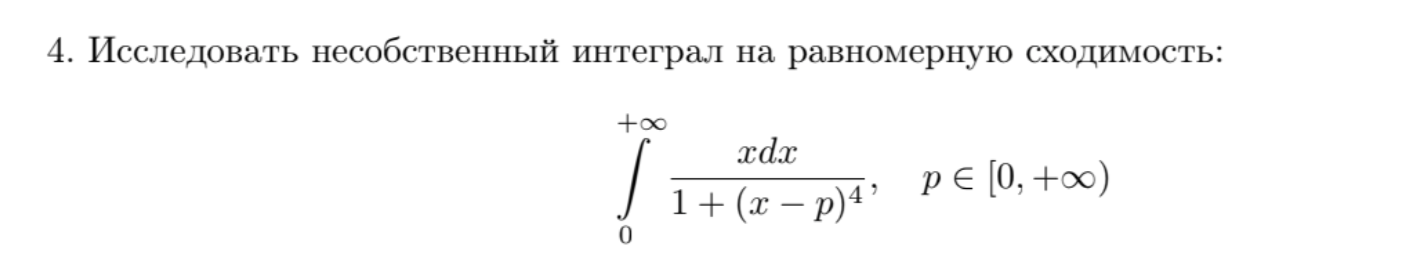
\includegraphics[scale=0.5]{4.png}
\end{center}
Колесниченко сказала, что в дз где-то будет признак Коши, значит юзаем признак Коши:
\begin{center}
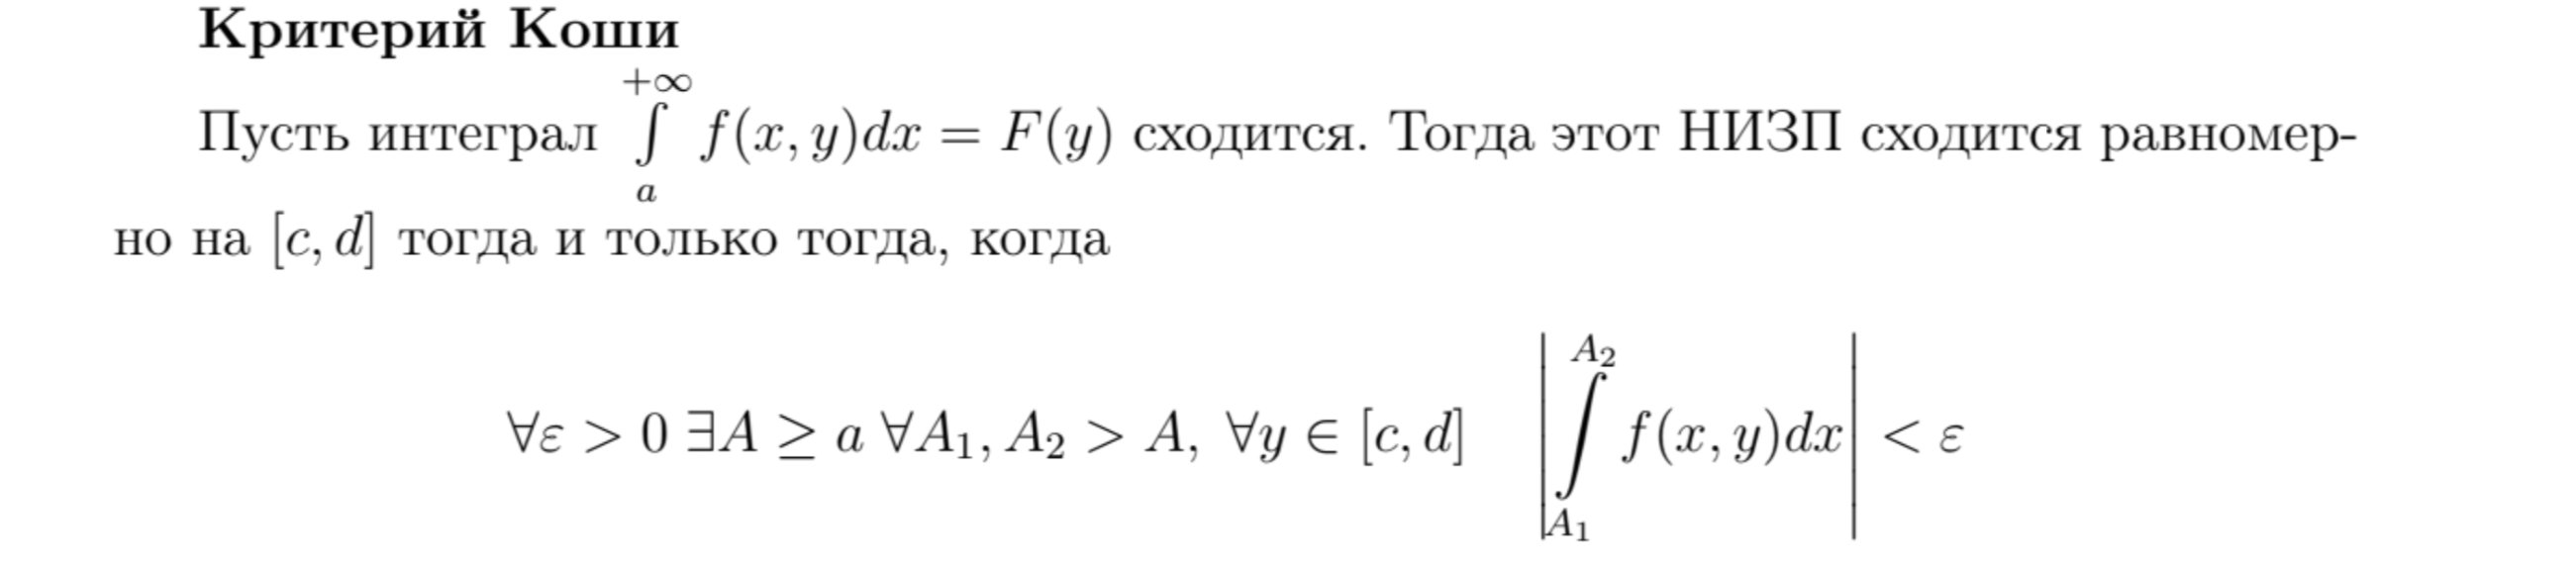
\includegraphics[scale=0.3]{koshi.png}
\end{center}
Делаем аналогично 3му номеру с сема. Хотим сделать числитель минимальным, знаменатель максимальным. Тогда в числитель нужно подставлять $A_1$, а в знаменатель что подставлять непонятно. Тогда условимся, что $(A_1 - p)^4 > 	(A_2 - p)^4$, чтобы не рассматривать два аналогичных случая (в силу возможности выбора $p$, $A_1$, $A_2$ там всё будет также):
\[
\left|
\int_{A_1}^{A_2} \frac{xdx}{1 + (x - p)^4}
\right|
\geq 
\frac{A_1}{1 + (A_1 - p)^4}
\int_{A_1}^{A_2}  dx  
=
\frac{A_1}{1 + (A_1 - p)^4}
(A_2 - A_1)
=
\]
Аналогично сему берем $A_2 = 2A_1$:
\[ 
=
\frac{A_1}{1 + (A_1 - p)^4}
A_1
=
\]
Теперь берем $p = A_1$:
\[
=
\frac{A_1^2}{1 + (A_1 - A_1)^4}
=
\frac{A_1^2}{1}
=
A_1^2
\]
Тогда берем отрицание Коши:
\[
\forall A_0 > 0 \; \exists \; A_1, A_2 = 2A_1 > A_0 \; \exists \; p = A_1 : 
\left|
\int_{A_1}^{A_2} \frac{xdx}{1 + (x - p)^4}
\right| \longrightarrow \infty
\]
А значит нет равномерной сходимости
\begin{center}
\textbf{Ответ:} расходится
\end{center}
\end{document}
